%************************************************
\chapter{Data Analysis at the LHC}\label{ch:introduction}
%************************************************
The LHC produces about 40 millions bunch crossings per second in the various interaction points. The detector has roughly 100 millions acquisition channels, meaning that if one was to read all of them for each event, it would need around \emph{4 PB/s of raw data} for storing all the events. The actual amount of data collected for each event, including pile-up, is around 1 MB (1 Megabyte), thanks to \emph{zero suppression}, which discards channels with a signal below the noise treshold in the apparatus. This means that we are reaching 40 TB/s of data--far too much for any conventional data acquisition system to handle.

The trigger systems alleviate the problem by reducing the amount of data by a factor or 10$^{4}$, hence to 4 GB/s. Despite this, the constant need of cutting-edge resources and solutions, both in hardware and software, have been driving extremely fruitful research in the history of the LHC.

One major necessity, whose importance and scale may not be appreciated by people outside of the field, is the one for \emph{simulations}. We explain the concept more in detail in the following, drawing from \cite{sims} as an informal reference.

\section{The necessity of simulations}

Before starting, we have to understand why do we need simulations in the first place.
The simulation is a crucial aspect of any high energy physics experiments. In CMS it is used both
at analysis level and for testing the algorithms before deployment with data. 
Simulations help in a wide range of scenarios:

\begin{outline}
   \1  The simulation can provide us with detailed predictions of the expected SM processes, allowing us to optimize our analysis according to the theoretical expected signatures. It can also target relatively rare processes originating from a hard interaction between two proton components, which are signal or background for specific analyses;


\1 Additionally, thanks to simulation we are able to study the performance of the detector on reconstruction algorithms, crucial for proper data taking.
\end{outline}
\section{Modelling an event} \label{sec:modelling}

There are three major, distinct steps in modelling a physical event at CMS. The first one,  \emph{generation}, is more generally related to the physical theories and calculations, while the other two, \emph{simulation} and \emph{digitization}, are specific to the CMS detector. The whole process is often referred to as \emph{FullSim} (full simulation).

\subsection{Event generation}

The first step to simulation is called generation, and it is based on the theoretical calculations which describes how the quarks and gluons inside the protons scatter off one another, how they might create new particles, and how those new particles behave after they have been created. 

Proton-proton collisions are very complex and difficult to model accurately. Protons are
composed of 3 quarks, called \emph{valence} quarks, by virtual gluons and virtual quark anti-quark
pairs coming from gluon splitting. All constituents of hadrons are generically called \emph{partons}.
During high energy collisions, the protons behave as a collection of free partons and the
hard scattering can be described at the level of parton interactions. The hadronic cross
section $\sigma_{pp}$ is calculated based on the QCD \emph{factorization} theorem. The factorization theorem
states that the hadronic cross-section $\sigma_{pp}$ is a convolution of the partonic cross section  $\hat{\sigma}_{ij}$ with the parton distribution functions (PDFs) $f_i(x)$:

\[
\sigma_{pp} = \int_{x_{min}}^1 dx_1 dx_2 \sum_{i,j}f_i(x_1)f_j(x_2)\hat{\sigma}_{ij}(x_1 p_1, x_2 p_2)
\]

where function $f_i(x)$ is probability density that a parton of type i has a fraction x of the
hadron energy. The final cross section may be evaluated by the single, non-trivial contributions $\hat{\sigma}_{ij}$.

Apart from the hard interactions, i.e. parton-parton interactions with large momentum transfer which results into high-momentum final-state particles, the other constituents of the proton can also interact. This
usually results in a collection of softer particles, called \emph{underlying event} (UE). High momentum quarks and gluons involved in the collision will emit additional hard QCD radiation. Radiation
from particles before the hard interaction is called \emph{initial-state-radiation} (ISR), whereas radiation off particles produced in the collision is called \emph{final-state-radiation} (FSR). All the quarks
and gluons go through the hadronization process, forming colorless hadrons. Finally, unstable particles are going to decay. A representation of all these elements is shown in Figure \ref{fig:evgen}.          

\begin{figure}
    \centering
     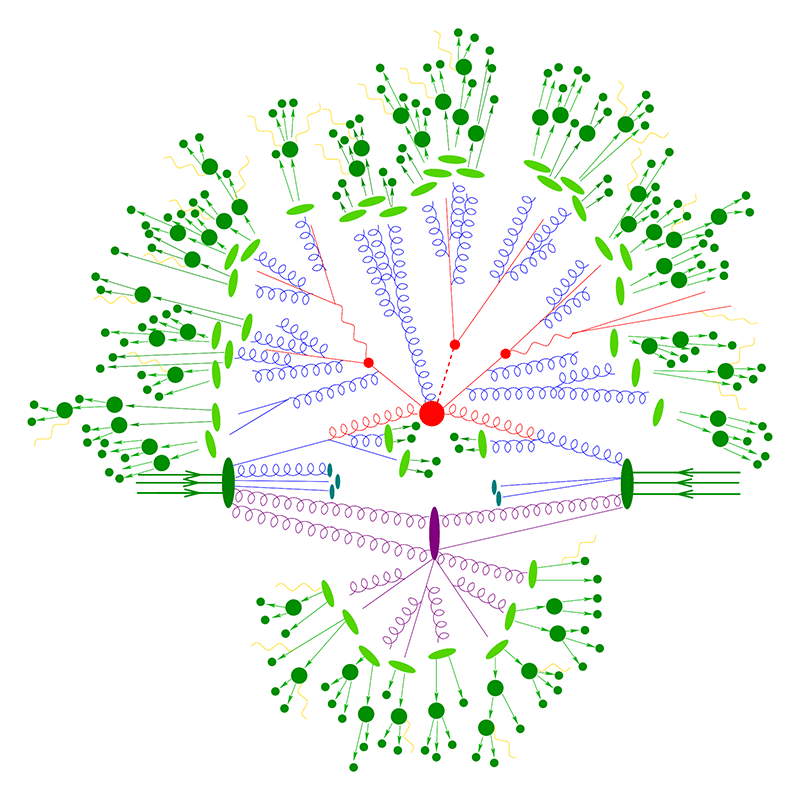
\includegraphics[width=.65\linewidth]{gfx/ch2/event_800px.png}
    \caption[Event generation]{ We can get a better understanding of a proton-proton collision event through this visualization. The red part includes the hard interaction and the decay of the products. Initial and final state radiation are in blue. A secondary
interaction can take place, in purple, before the final-state partons hadronize. The hadronization is
represented by the green blobs, and the hadron decay in dark green. Photon radiation is in yellow. From \cite{evgen}.}
    \label{fig:evgen}
\end{figure}


All the various parts involved in this step can be summarized as:

\begin{outline}
    \1  The PDFs that are phenomenological functions computed using experimental information;
    \1  the hard scattering, computed perturbatively order by order;
    \1  the parton \emph{showering}, used to simulate additional emissions in perturbative QCD;
    \1   the hadronization, describing the transition from colored particles to hadrons, treated
        using phenomenological models;
    \1   the decay of unstable particles, modeled based on experimental data.
    
\end{outline}

The first two are usually included in \emph{Matrix Elements generators}, while the last three are
included in Parton Showering programs. Both use Monte Carlo techniques; some popular multi-purpose generators include \texttt{Pythia8} \cite{Bierlich:2022pfr}, \texttt{MadGraph} \cite{Alwall_2014} and \texttt{Sherpa} \cite{Bothmann_2019} as well as \texttt{POWHEG} \cite{Nason_2004} and \texttt{MadGraph5\_aMC@NLO} \cite{powpow}, wich will be more relevant in the following chapters.

We can thus obtain a complete description of all the (stable) particles that come out of a collision between two protons under our theory only after a complex process involving several steps of modelling and calculations. At the end of this process a generated event is just a list of the particles produced and their kinematic properties.


\subsection{Detector Simulation through GEANT4}

Now that we have the particles resulting from our process, we must take the detector into account. This means simulating all the interaction processes that are going to happen between particles and matter by moving them through the detector one by one and modelling the detector’s response to each one of the particles as it goes. 
Undoubtedly, the de-facto standard for such a task is the \texttt{Geant4} toolkit (see \cite{AGOSTINELLI2003250}). It is intended to simulate the passage of particles through matter and it includes a complete range of functionality including keeping track of where particles have passed, geometry, physics models and hits. The physics processes offered cover a comprehensive range, including magnetic field interactions, hadronic and optical processes, a large set of long-lived particles, materials and elements, over a wide energy range starting, in some cases, from 250 eV and extending in others to the TeV energy range. It has been designed and constructed to expose the physics models utilised, which describe each process (e.g. the photoelectric effect, Compton scattering, bremsstrahlung, ionization, multiple scattering, decays, nuclear interactions, $\dots$) for each particle. Additionally it can handle complex geometries, and enable its easy adaptation for optimal use in different sets of applications. The toolkit is the result of a worldwide collaboration of physicists and software engineers, created exploiting software engineering and object-oriented technology and implemented in the \texttt{C++} programming language.

\begin{figure}
    \centering
     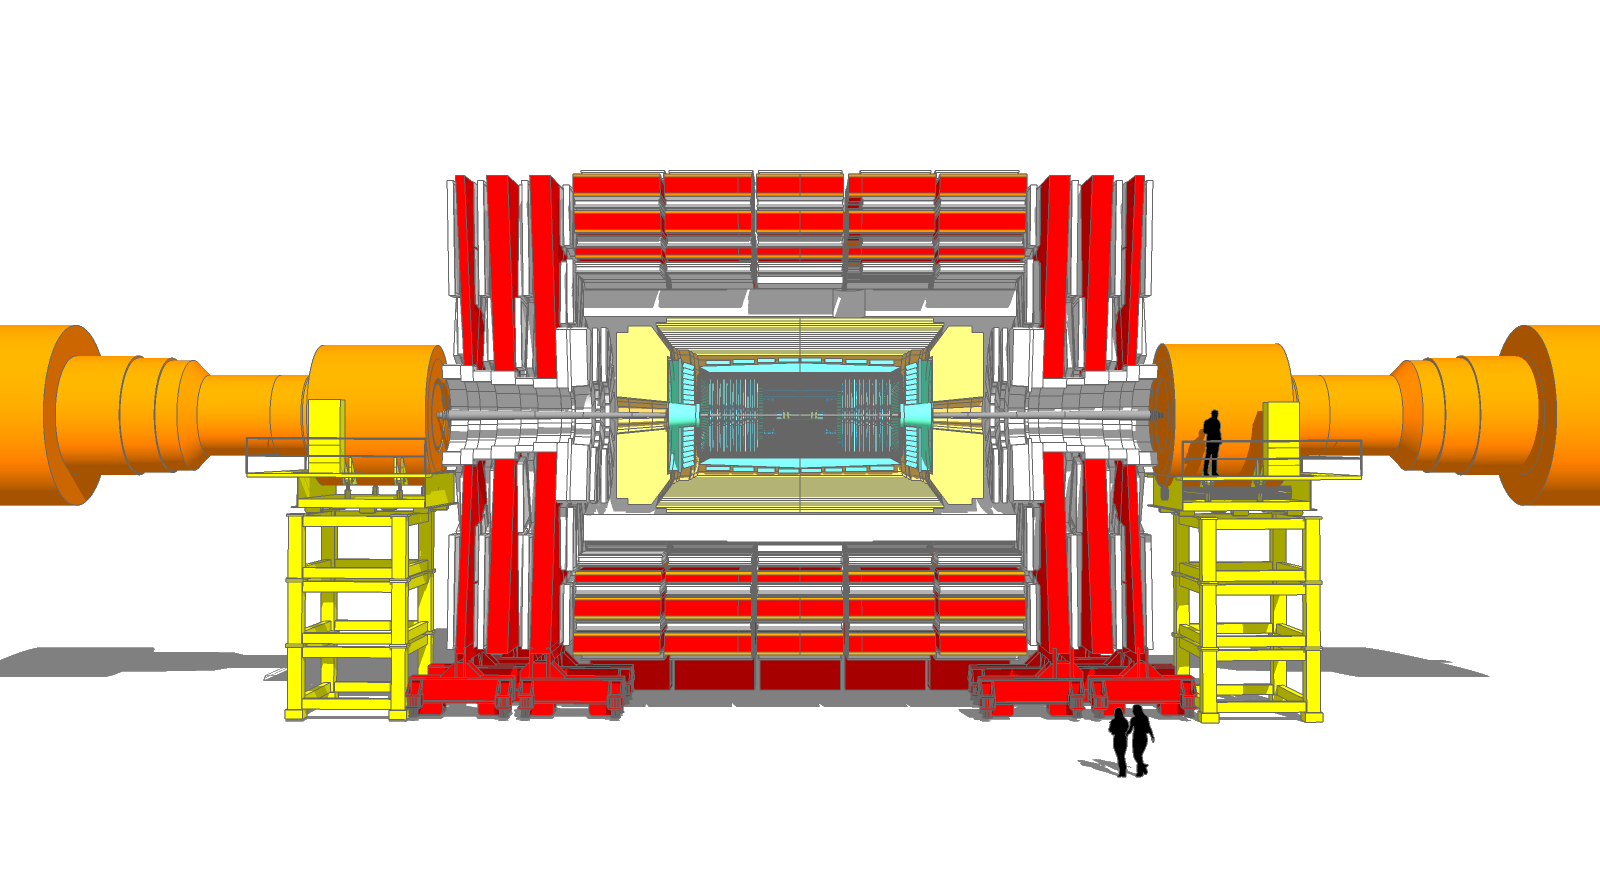
\includegraphics[width=\columnwidth]{gfx/ch2/cms_160518_01_Scene_2.png}
    \caption[CMS model]{ This representation of the CMS detector is based on the actual \texttt{Geant4} CMS Detector Description discussed in the text. It accurately and precisely reproduces the geometry of all CMS detector subsystems, including the geometries of the original CMS detector, phase 1 and phase 2 upgrades.  From \cite{decmod}.}
    \label{fig:decmod}
\end{figure}


However, \texttt{Geant4} can only provide us with a description of the single physical processes and materials, so we need to provide the actual \emph{detector description} (see Figure \ref{fig:decmod}). 

Every piece of the detector has to be put together, with the right material assigned to each. The full detector description has millions of volumes and hundreds of different materials.

Finally, we specify the parts of the detector that are the most crucial, called \emph{sensitive} detectors. In the end we want to save all the energy deposits that  \texttt{Geant4} has made, their time and location – and sometimes information (called \emph{truth}) about what exactly happened in the simulation, so later we can find out, for example, how good our reconstruction software was at correctly identifying photons and their conversions into electron-positron pairs.

At the end of this costly step, we are left with a long list of energy deposits, times, and locations in our detector. 

\subsection{Digitization} 

The last part of the simulation process consists in turning the energy deposits into the actual signal outputted by the detector-- a process called digitization, once again specific for a given detector.

The simple idea is to change the energies into the detector outputs – usually times, voltages, and currents, for example. We have to build in all the detector effects that we care about. Some are well known such as Birks’ law, for example; others are more complicated, like the change in light collected from a scintillator tile in the calorimeter depending on whether the energy is deposited right in the middle or on the edge. We can use the digitization to model some of the very low-energy physics that we don’t want to have to simulate in detail with \texttt{Geant4} but want to approximate to an average. Those are effects like the spread and collection of charge in a silicon module or the drift of ionized gas towards a wire.

Digitization is where some other effects are put in, like the pile-up, the extra proton-proton collisions in a single bunch crossing. We can add other background effects if we want to, like cosmic rays crossing the detector, or proton collisions with remnant gas particles floating around in the beampipe, or muons running down parallel to the beamline from protons that hit collimators upstream. 
At the end of the process we have something that looks exactly like the real data – except we know exactly what it is, without any ambiguity.

\subsection{Reconstruction}
Finally, we also have to pass both our simulated data and the real data readouts to all the reconstruction algorithms of Section \ref{sec:offreco} to obtain a collection of physical objects as reconstructed by the detector readout. This is the \emph{reconstruction} step, resulting in events similar to the one shown in Figure \ref{fig:cmsev}.

\begin{figure}
    \centering
     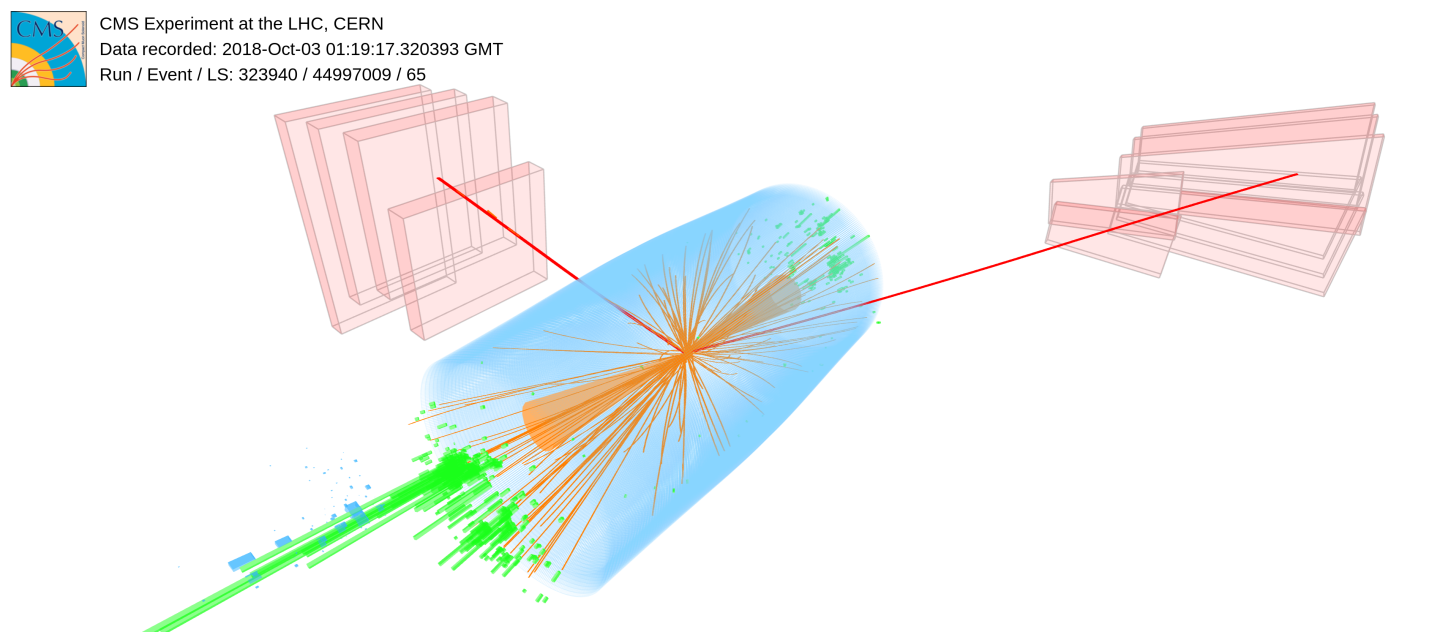
\includegraphics[width=\columnwidth]{gfx/ch2/HIG-19-006_VBF_white.png}
    \caption[CMS Event]{As an example of the final high-level event description, we show a final event description  where a candidate Higgs boson produced by vector boson fusion (VBF) decays into two muons, with an invariant mass of 125.01 GeV and per-event mass uncertainty of 1.83 GeV. The forward jets from the VBF are depicted by the orange cones and the muons are drawn as long red lines. Courtesy of the CMS Collection.}
    \label{fig:cmsev}
\end{figure}


Performing all the previous steps, we can simulate all sorts of different processes, like the production of top quarks, W bosons, Z bosons, the Higgs bosons and potentially new theoretically predicted processes. The last part, which is really what much of the data analysis is concerned with, is trying to figure out what makes events under the new hypothesis different from the other ones we expect to see – and trying to isolate them from the others. We can look at the reconstructed energy in the event, the number of particles we find, any oddities like heavy particles decaying away from the collision point – anything that helps. And we have to know potentially relevant information about the simulation, so that we do not end up using properties of the events that are very hard to simulate to separate new particles from known ones. 

Even if sometimes it can be useful to use \emph{data-driven} methods to estimate the backgrounds (or tweak the estimates from our simulation), it is common to start from the simulation itself to get a proper understanding of the expected background processes and their signals in the apparatus.

\subsection{Computing Costs}

Due to the length and the complexity of the process, its tremendous computation costs should not come as a surprise. In 2019, the final resources employed \emph{exclusively at CMS} were as follows:

\begin{outline}
    \1 7 PB of RAW data (including backup copies) and 3.5 PB of reconstructed data, 14 PB or RAW Monte Carlo and 7 PB of reconstructed simulation, for a total of 40 PB in a year;
    \1 The CPU resources employed in the end amounted to 70,000 cores, divided as follows:
    \2 10,000 cores for \emph{data reconstruction};
    \2 40,000 cores for Monte Carlo SIM and RECO steps;
    \2 20,000 for all the analysies (considering all the MC and data taking steps).
\end{outline}

As the luminosity increases and hence the PileUp, all these figures are expected to increase.
Figure \ref{fig:cpuusage} shows the public approved HL-LHC CMS projections for the CPU usage at CMS.

\begin{figure}
    \myfloatalign
    \subfloat[]
    {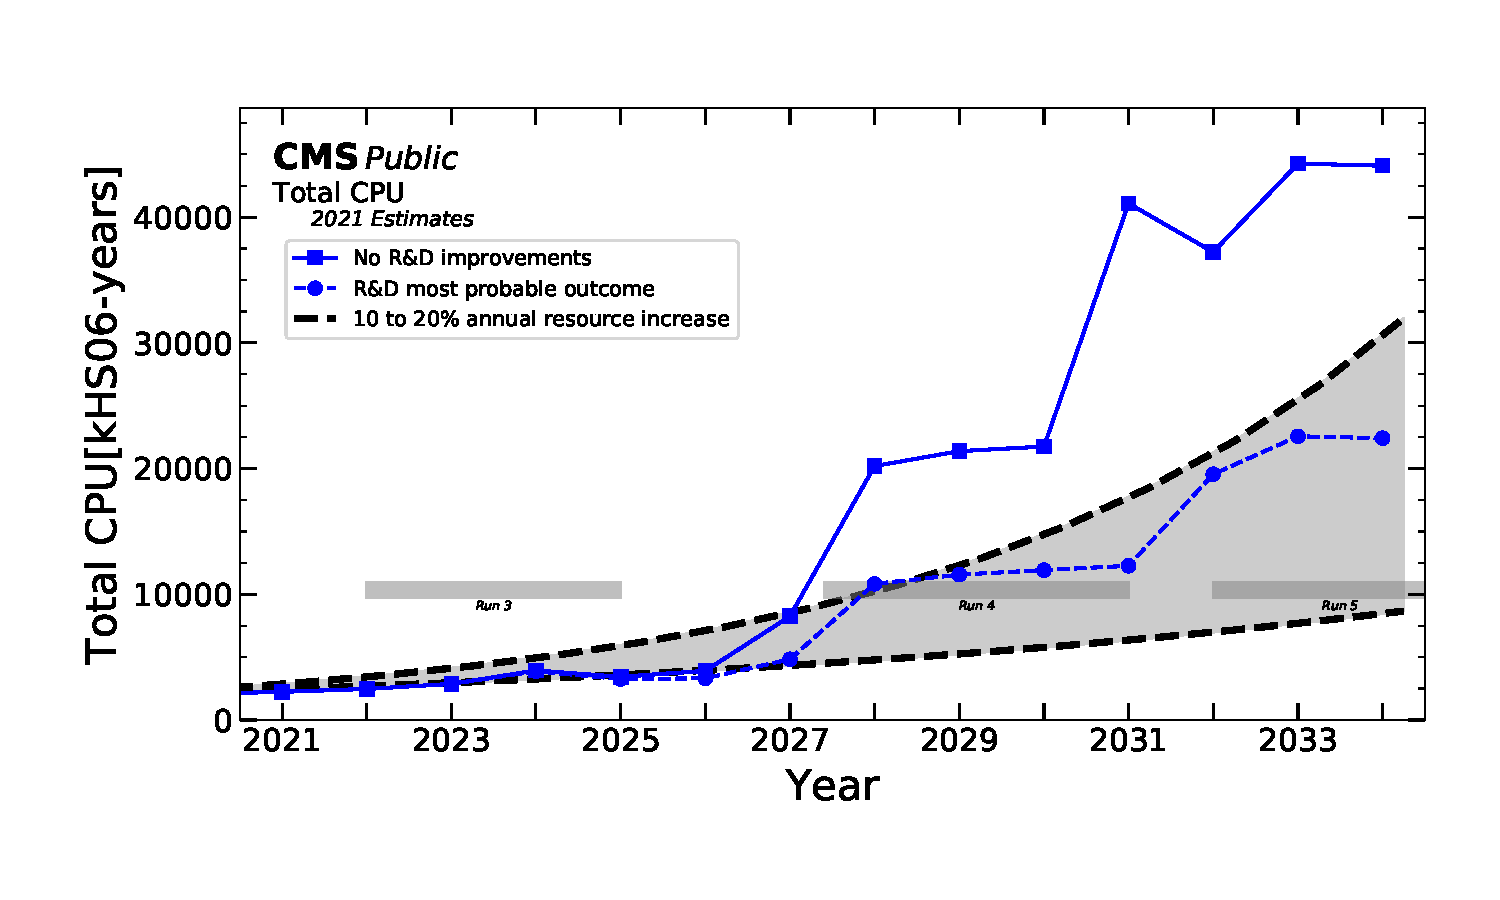
\includegraphics[width=.65\columnwidth]{gfx/ch2/cpu_cms2021.pdf}} \\
    \subfloat[]
    { 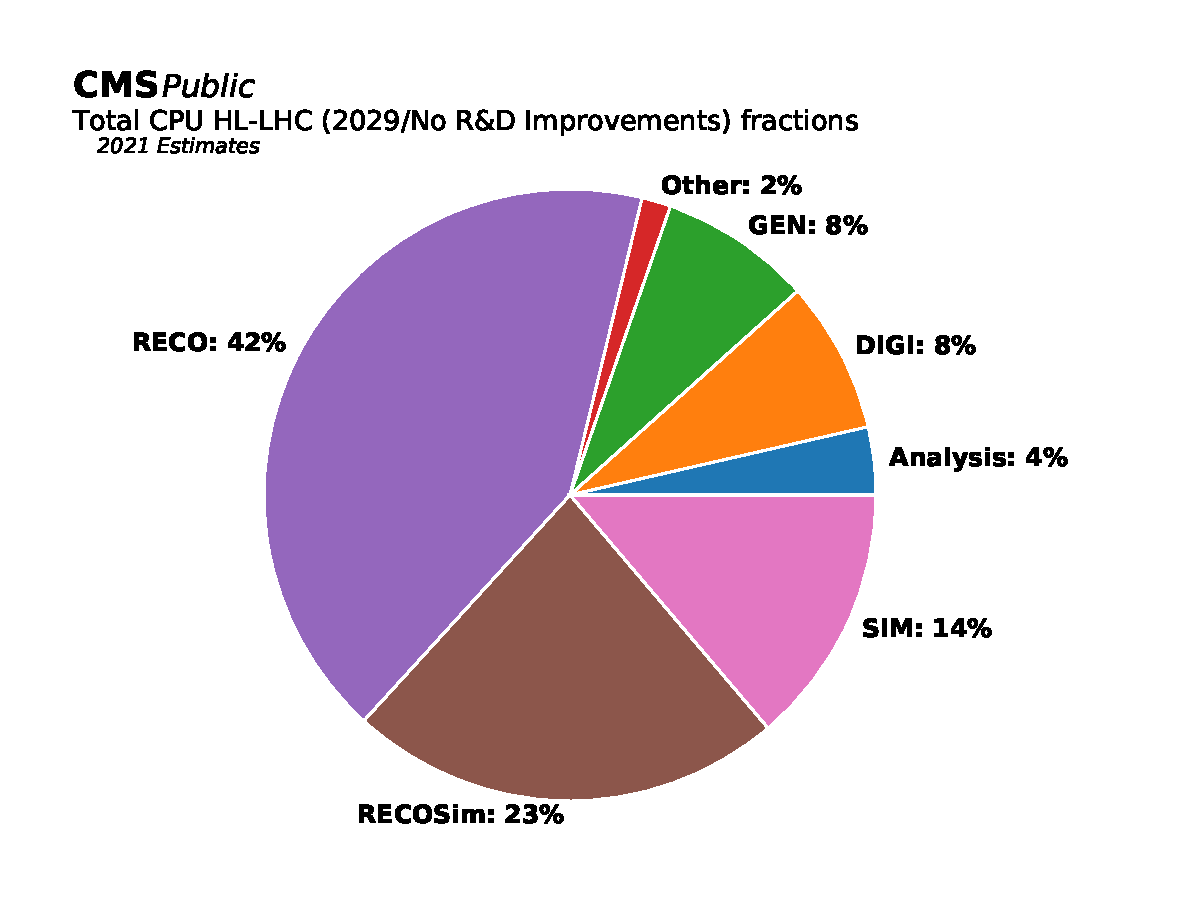
\includegraphics[width=.65\columnwidth]{gfx/ch2/cpu_pie_cms2021.pdf}} 
    \caption[Computing estimates]{The R$\&$D are necessary for the future of the experiment, as showed by the total CPU utilization projections (a) and the approximate breakdown of CPU time into primary processing and analysis activities (b) for the CMS experiment.}\label{fig:cpuusage}
\end{figure}

The plots show estimates from 2021 made for the CMS contribution to the LHCC November review of HL-LHC computing and common software, which supersede previous results from CMS. Coherently with the CMS Phase-2 Upgrade HLT TDR, an integrated luminosity of up to 350 fb$^{-1}$ per year at 200 pileup events (7.5 KHz high level trigger rate) is considered for future Runs. Two scenarios are considered: the first one is a baseline, which does not include any improvement due to ongoing R\&D activity, and the second one incorporates the most probable outcome of the ongoing R\&D activities. The blue curves (and points) show the annual projected needs, summed across Tier-0, Tier-1 and Tier-2 resource needs in each of these scenarios. The gray band shows the projected resource availability for an example scenario that extrapolates the 2018 CMS pledged resources using an annual increase in available resources of between 10$\%$ and 20$\%$. Results are derived from a bottom-up model of CMS offline processing activities, including prompt reconstruction, Monte Carlo simulation, data re-reconstruction and all phases of analysis activities. 

We also show the approximate breakdown of CPU time into primary processing and analysis activities during an hypothetical HL-LHC year. The plot corresponds to a snapshot of the year 2029. The baseline scenario is considered, i.e. projected effects from on-going R\&D that will reduce the computing resources needed by CMS are not considered.

The presented figures make it clear that:

\begin{outline}
    \1 Both the future and the present CPU (as well as Disk) utilization are mainly employed for the event simulation tasks, which leaves out about 48$\%$ of resources for other necessities;
    \1 Without improvements from the R\&D sector we risk not being able to meet the future scientific goals.
\end{outline}


\subsection{Fast simulation}\label{sec:fastsim}

Clearly, the possibility of performing fast simulations would be a major improvement over the current simulation pipeline, and there are already many different studies and approaches for doing so.

\paragraph{Simplifying the interactions}

In this type of approach, we search for the slowest part of our process and find ways of making it as fast as possible with specific parametric shortcuts. The CMS Collaboration currently has a dedicated approach called CMS \emph{FastSim}, see \cite{https://doi.org/10.48550/arxiv.1701.03850}. 

While FullSim uses the exact detector geometry, tracks particles in small steps, and uses
detailed models for material interactions, FastSim uses a simplified geometry with simple analytical material interaction models that are parametrized
and tuned to agree with FullSim. For the digitization step, both FullSim and FastSim do a detailed
emulation of detector electronics and trigger, with small exceptions in FastSim. In the reconstruction step, FullSim employs the standard event reconstruction used for reconstructing the real CMS
data. FastSim uses standard reconstruction for calorimetry and muon systems, but a simplified
reconstruction for tracking, based on smearing and truth information, in order to reduce CPU time. Downstream reconstruction and definition of analysis objects is the same as that used by real data and FullSim.

Performance of FastSim is validated regularly within the official CMS software release validation framework; overall, distributions in FastSim agree with FullSim within $\approx 10\%$ \cite{https://doi.org/10.48550/arxiv.1701.03850}. See Table \ref{tab:simfram} for a quick comparison with the others simulation approaches.

\paragraph{Starting from final-state generator objects}

In this kind of approach we try to skip detector simulation and digitization all together and go directly to the final objects that we would have reconstructed (electrons, muons, jets, missing transverse momentum, $\dots$). A popular framework is the one of \texttt{DELPHES} fast-simulation, see \cite{de_Favereau_2014}.

It takes as input the final-state output of an event generator and performs a fast and realistic simulation of
a general purpose collider detector. To do so, long-lived particles emerging from the hard
scattering are propagated to the calorimeters within a uniform magnetic field parallel to
the beam direction. The particle energies are computed by smearing the initial long-lived
visible particles momenta according to the detector resolution. As a result, jets, missing
energy, isolated electrons, muons and photons, and taus can be reconstructed. It is oviously not meant to
be used for advanced detector studies, for which more accurate tools are needed, but it can nonetheless perform quickly realistic physics studies without in-depth knowledge of the technicalities. It should be noted that this type of strategy currently makes up the HL-LHC studies workhorse, as it is capable of providing acceptable results in a fraction of the time needed by the other approaches. It should be noted that the content of a \texttt{DELPHES}' simulated event is also different from what is typically used in detector-data analyses and from the results of Full/FastSim. 


\begin{table}
\begin{adjustbox}{width={\textwidth},totalheight={\textheight},keepaspectratio}%
    \begin{tabular}{llll} \toprule
        \tableheadline{Simulation framework} & \tableheadline{key aspects} & \tableheadline{speed} & \tableheadline{accuracy/limitations}\\ \midrule
        FullSim & \tabitem detailed geometry; &  $\mathcal{O}(40$ s) for a t$\overline{\text{t}}$ event &\tabitem Best\\
        & \tabitem small-step tracking; & &\\
        & \tabitem \texttt{Geant4} material modelling; & &\\
        & \tabitem  detailed digitization; & &\\
        & \tabitem full reconstruction & &\\
        \midrule
        FastSim & \tabitem simplified geometry; &  $\mathcal{O}(5$ s) for a t$\overline{\text{t}}$ event & \tabitem Lacks \emph{fake tracks}; \\
        & \tabitem thin material layers; & & \tabitem skips track and reco steps;\\
        & \tabitem simple analytical material modelling; & &\tabitem some analysis data (e.g. trigger) not available\\
        & \tabitem  detailed digitization; & &\\
        & \tabitem full reconstruction with exceptions & &\\
        %postulant quo & westeuropee & sanctificatec \\
        \midrule
        Delphes & \tabitem simple tracking system; &  $\mathcal{O}(0.01$ s) for a t$\overline{\text{t}}$ event & \tabitem Limited reco pair correlations;  \\
        & \tabitem smearing & & \tabitem 1-d smearing;\\
        & & & \tabitem different analysis data format w.r.t. Full/FastSim\\
        %autem vulputate ex & parola & romanic \\
        %usu mucius iisque & studio & sanctificatef \\
        \bottomrule
    \end{tabular}
    \end{adjustbox}
    \caption[Simulation frameworks]{An at-glance comparison between the various simulation frameworks employed at the CMS experiment, useful for understanding the current approaches.}
    \label{tab:simfram}
\end{table}

As Table \ref{tab:simfram} shows, the various fast simulation approaches allow us to obtain significant speedups. However, while CMS FastSim accuracy is constantly being improved, its speed is still somewhat lacking; while \texttt{DELPHES} achieves a marked speedup but sacrifices the realistic detector simulation.

\section{The standard CMS Analysis format: NanoAOD}\label{sec:nanoaod}

Because the simulation consists of so many different steps, we end up with a large amount of information for each event. Aside from final state objects, we are able of keeping track of various steps as the particles pass through the detector, as well as individual components of jets, with great precision. Starting from raw data produced from the online system or the MC full simulation, successive degrees of processing (the event reconstruction) refine this data, apply calibrations and create higher-level physics objects. CMS uses a number of data formats with varying degrees of detail, size, and refinement to write this data in its various stages. In turn, the data formats get grouped within an Event file into multiple Event formats, according to the data origin or content. Because of this the \emph{size} of the resulting output is larger than what is typically needed by the analyses.

Event information from each step in the simulation and reconstruction chain is logically grouped into what we call a \emph{data tier}. Examples of data tiers include RAW and RECO, and for simulated data we also have the previously mentioned steps: GEN, SIM and DIGI. A given dataset may consist of multiple data tiers, e.g., the term GenSimDigi includes the generation (MC), the simulation (Geant) and digitization steps. The most important tiers are probably RECO (all reconstructed objects and hits) and AOD (Analysis Object Data, a smaller subset of RECO). Figure \ref{fig:datatier} gives an overview. 

\begin{figure}
    \centering
     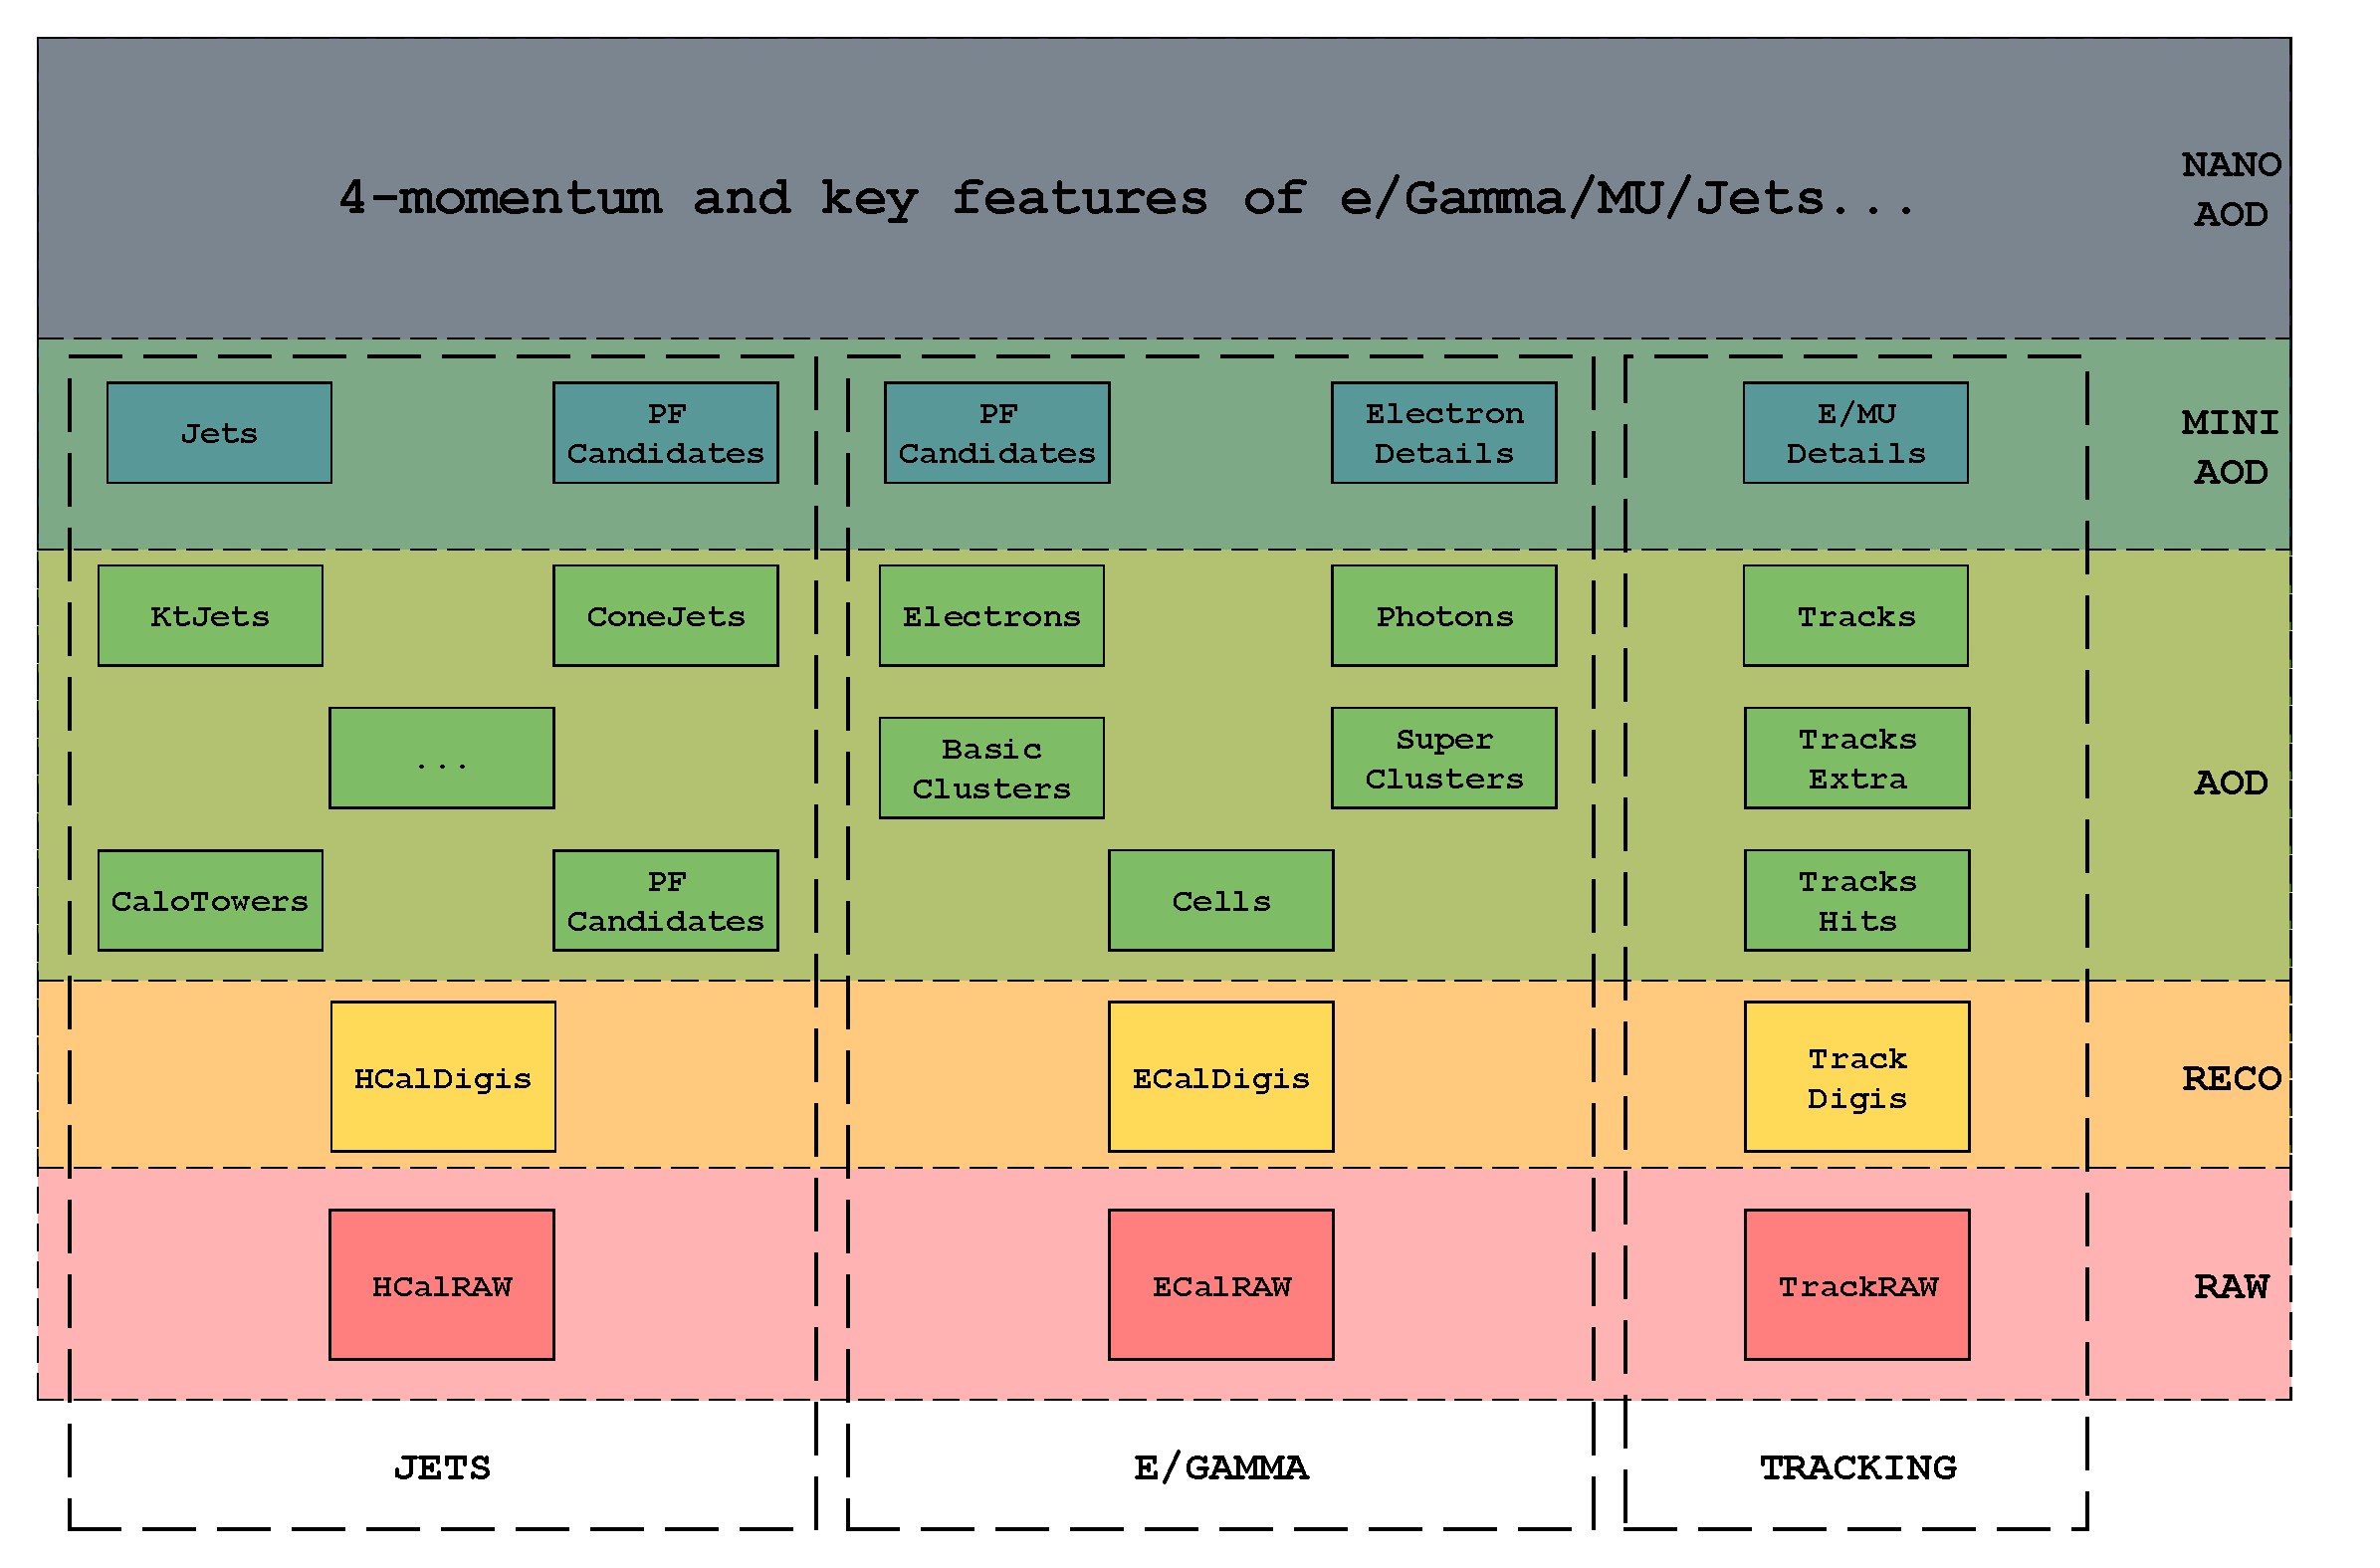
\includegraphics[width=\columnwidth]{gfx/ch2/data_tiers.pdf}
    \caption[Data Tiers]{RAW data is the Detector data after online formatting, the L1 trigger result, the result of the HLT selections (HLT trigger bits), potentially some of the higher level quantities calculated during HLT processing. RECO data contains objects from all stages of reconstruction. AOD are derived from the RECO information to provide data for physics analyses in a convenient, compact format. MiniAOD and NanoAOD do the same, returning a progressively smaller format. Most physics analyses can run on either MiniAOD or NanoAOD data.}
    \label{fig:datatier}
\end{figure}

The AOD format, containing all the relevant physical objects, formed the backbone of the CMS analyses for the entirety of Run 1. However, such an amount of information mean that the typical AOD will store about 400 kB \emph{per event}. This is often redundant for the needs of analysis. Additionally, the increase in luminosity during subsequent runs means that the size of the format will keep increasing: at the end of 2013, the total size of AOD stored by CMS for Run 1 was about 20 petabytes. The CMS collaboration has thus commissioned various new data formats aimed at reducing the size of the analysis data files.
Initially the MiniAOD format was introduced in 2014 (see \cite{Petrucciani_2015}), about one tenth the size of AOD (i.e. 40-60 kB per event), and which has seen a wide adoption by the experiment during Run 2. In recent years, however, the \emph{NanoAOD} format has been proposed \cite{Rizzi:2699585}, with the aim of serving the needs of a substantial fraction of CMS physics analyses with a per-event payload of about 1-2 kB.

NanoAOD achieves such a strong data reduction by retaining only high level information on physics objects, such as jets and leptons, dropping their individual constituents, and reducing the precision of stored variables.
The design rationale of NanoAOD is based on previous experience from \emph{user "ntuples"} and considerations on which minimal set of object information can support a large set of analysis efforts. The introduction of the NanoAOD data format has a dramatic impact on the estimates for computing resources needed by the CMS experiment during the High-Luminosity operation phase of the LHC. Assuming a design target of 50$\%$ analysis coverage with NanoAOD is met by then, the projected needs for disk storage in 2027 are decreased by a factor of about 2, corresponding to a reduction of more than 2 EB (Exabytes). The needed CPU processing power is also decreased by about 15$\%$, as user ntuple production is partially replaced by the central NanoAOD workflow. 

The full content of a NanoAOD file may be found \href{https://cms-nanoaod-integration.web.cern.ch/integration/master-102X/mc102X_doc.html}{here}\footnote{\url{https://cms-nanoaod-integration.web.cern.ch/integration/master-102X/mc102X_doc.html}}. The NanoAOD format contains a \texttt{TTree} data structure made up of several Events, each consisting of multiple final-state physical objects useful for the analysis, such as the Jet, Muon, Tau and PileUP objects, as well as a series of Gen objects, that is the outputs of the Generation step discussed above. In this way, it may be possible to match the Gen object with its corresponding reconstructed counterpart, whose properties are expected to change after the interaction with the detector and the readout/reconstruction processes. It should be noted that the collections of reconstructed object will inevitably contain \emph{fakes}, not matched to any Gen level object due noise and PileUp.

Despite the great advantages, the potential of the NanoAOD for simulated data is still partially hampered by the current production procedure: NanoAOD can be produced from MiniAOD files at a rate of about 10 events per second on a
single CPU core. This, in turn, means that we are bound to have an underling AOD file, which implies that we still need to perform all the computationally expensive steps of Section \ref{sec:modelling} if we are to simulate our data.
However, the consistently reduced size of the NanoAOD opens up new possibilities for its production thorugh non-conventional, non-\texttt{Geant4} based approaches. 

Specifically, in the present work we are interested in investigating \emph{state-of-the-art deep learning} techniques as a way of bypassing the Simulation, Digitization \emph{and} Reconstruction steps and directly produce new, original events in the NanoAOD format starting from Gen-level information in a fraction of the time and using only a subset of the resources.

\begin{figure}
    \centering
    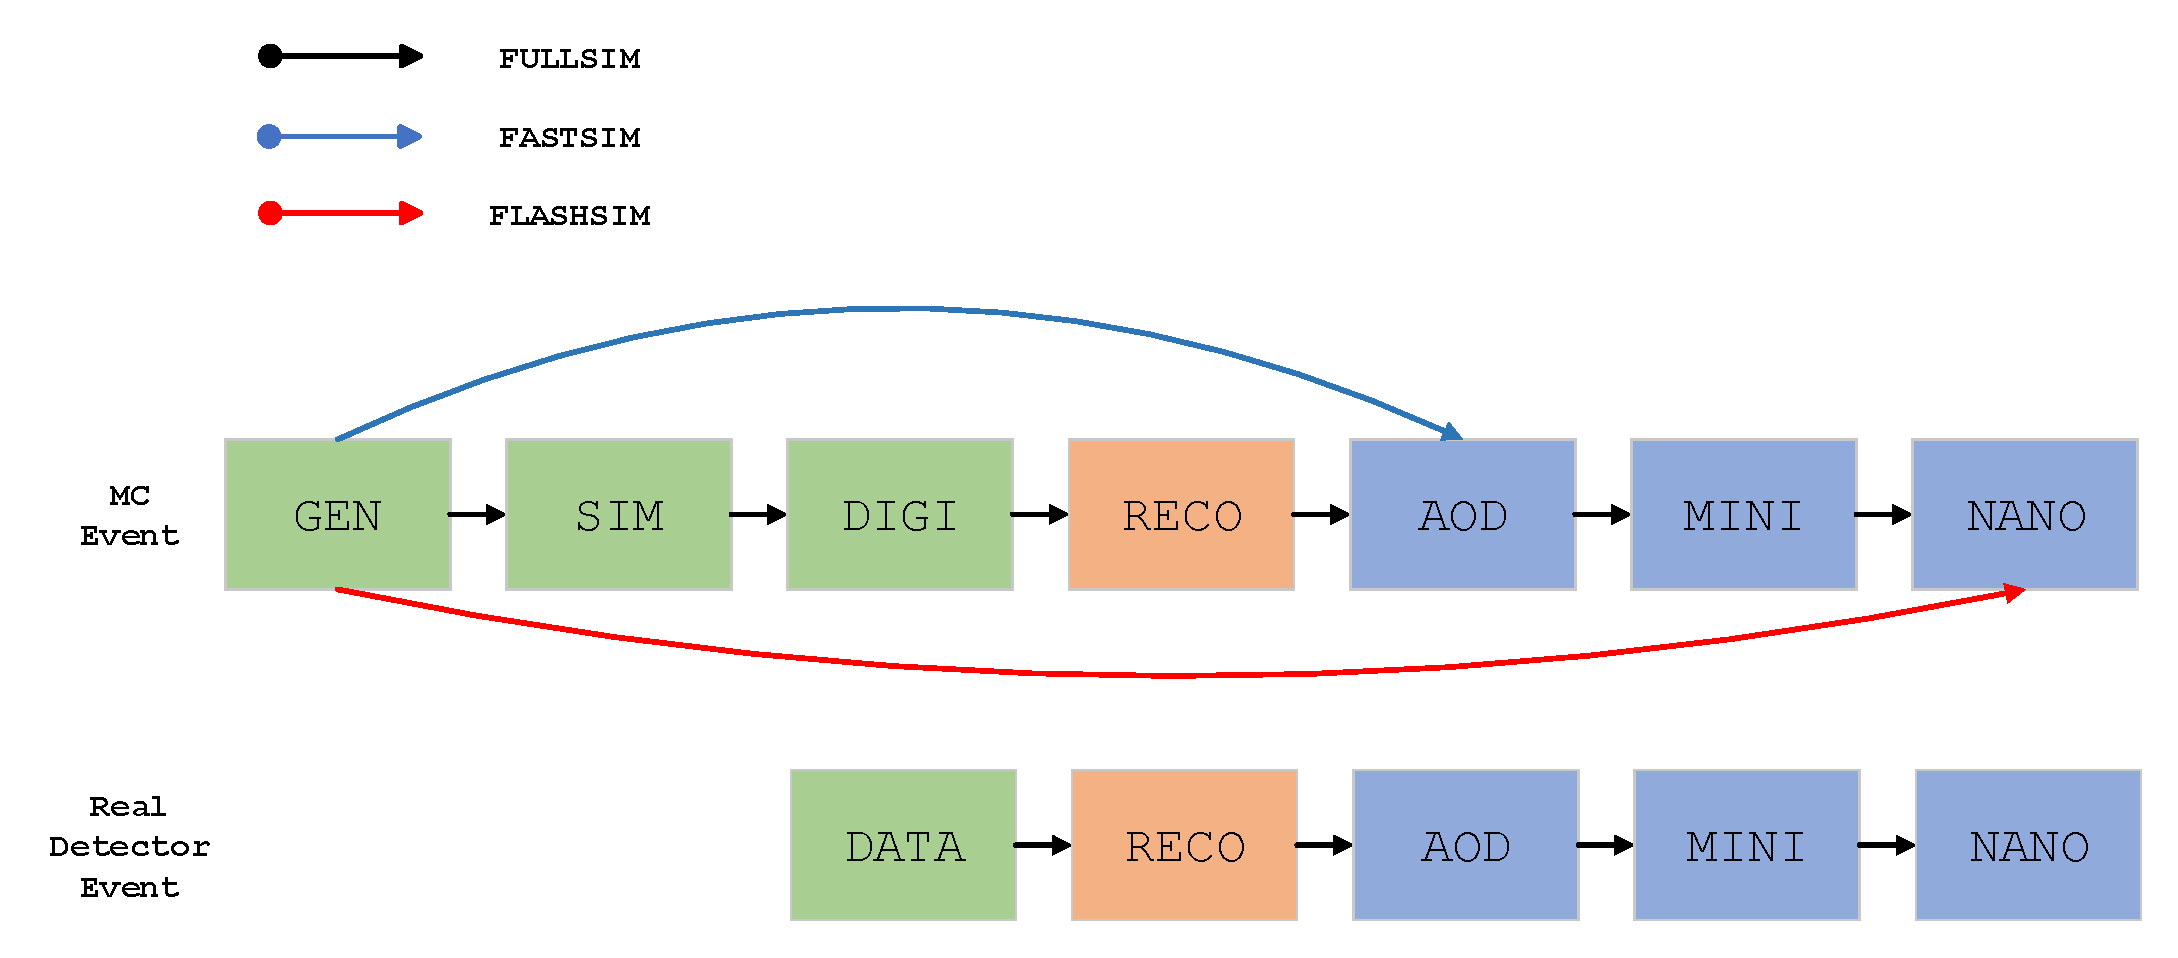
\includegraphics[width=\columnwidth]{gfx/ch2/sim_comp.pdf}
    \caption[Simulation comparison]{The proposed FlashSim would be able of performing realistic NanoAOD production and effectively bypassing all the intermediate steps. The FullSim chain is showed above, along with the CMS FastSim and our FlashSim approaches. We show below the real data processing chain: the RECO and file formats steps are in common between the two.}
    \label{fig:sim_comp}
\end{figure}

The idea behind this approach is simulating only the small set of variables present in NanoAOD, useful to perform physical analyses. This means that the overall complexity of the simulation target has been greatly reduced as we are not interested in precise track or hits reconstruction, for example. The goal is to reach a precision at least at the level of FastSim with a speed at least at the level of \texttt{DELPHES}.

As a final recap of this chapter discussion, we show in Figure \ref{fig:sim_comp} a comparison between the FullSim chain, the FastSim approach and our proposed FlashSim. The real data processing pipeline is also showed underneath.
%*****************************************
%*****************************************
%*****************************************
%*****************************************
%*****************************************
